%%%%%%%%%%%%%%%%%%%%%%%%%%%%%%%%%%%%%%%%%%%%%%%%%%%%%%%%%%%%%%%%%%%%%%%%%%%%%%%%
%2345678901234567890123456789012345678901234567890123456789012345678901234567890
%        1         2         3         4         5         6         7         8

\documentclass[letterpaper, 10 pt, conference]{ieeeconf}  % Comment this line out if you need a4paper

%\documentclass[a4paper, 10pt, conference]{ieeeconf}      % Use this line for a4 paper
\usepackage{graphicx}
\usepackage{amsmath}
\usepackage{algorithm}
\usepackage{algorithmic}
\usepackage{morefloats}
\usepackage{dblfloatfix}
\usepackage{amssymb}

\newcommand{\zmin}{z_{min}}
\newcommand{\zmax}{z_{max}}
\newcommand{\ddzcf}{\ddot{z}_{c,1}}
\newcommand{\ddzcs}{\ddot{z}_{c,2}}
\newcommand{\rcmpd}{\mathbf{r}_{cop,d}}
\newcommand{\rcmpr}{\mathbf{r}_{cop,r}}
\newcommand{\icpr}{\boldsymbol{\xi}_r}
\newcommand{\icp}{\boldsymbol{\xi}}
\newcommand{\icpe}{\boldsymbol{\xi}_e}
\newtheorem{lem}{Lemma}
\graphicspath{{figures/}}
\IEEEoverridecommandlockouts                              % This command is only needed if 
                                                          % you want to use the \thanks command

\overrideIEEEmargins                                      % Needed to meet printer requirements.

%In case you encounter the following error:
%Error 1010 The PDF file may be corrupt (unable to open PDF file) OR
%Error 1000 An error occurred while parsing a contents stream. Unable to analyze the PDF file.
%This is a known problem with pdfLaTeX conversion filter. The file cannot be opened with acrobat reader
%Please use one of the alternatives below to circumvent this error by uncommenting one or the other
%\pdfobjcompresslevel=0
%\pdfminorversion=4

% See the \addtolength command later in the file to balance the column lengths
% on the last page of the document

% The following packages can be found on http:\\www.ctan.org
%\usepackage{graphics} % for pdf, bitmapped graphics files
%\usepackage{epsfig} % for postscript graphics files
%\usepackage{mathptmx} % assumes new font selection scheme installed
%\usepackage{times} % assumes new font selection scheme installed
%\usepackage{amsmath} % assumes amsmath package installed
%\usepackage{amssymb}  % assumes amsmath package installed

\title{\LARGE \bf
Balancing using Vertical Center Of Mass Motion: A 2D Analysis from Model to Robot
%Vertical Center of Mass Motion for Balance Control: Capture Regions and Push Recovery on NASA's Valkyrie
}
\author{Boris J. van Hofslot$^{1,2}$% <-this % stops a space
\thanks{*This work was not supported by any organization}% <-this % stops a space
\thanks{$^{1}$The author is with the Florida Institute for Human and Machine Cognition, 40 S Alcaniz St, 32502 Pensacola FL, United States
        {\tt\small bvanhofslot@ihmc.us}}%
\thanks{$^{2}$The author is with the Department of Cognitive Robotics, Delft University of Technology, Mekelweg 2, 2628 CD Delft, Netherlands
        {\tt\small b.j.vanhofslot@student.tudelft.nl}}%
}


\begin{document}



\maketitle
\thispagestyle{empty}
\pagestyle{empty}


%%%%%%%%%%%%%%%%%%%%%%%%%%%%%%%%%%%%%%%%%%%%%%%%%%%%%%%%%%%%%%%%%%%%%%%%%%%%%%%%

%& ABSTRACT
\begin{abstract}
Balancing strategies for humanoid robots often include center of pressure control (`ankle' strategies), change of body angular momentum (e.g., `hip' strategies) and taking a step. We use vertical center of mass motion as an additional input for balance control. We walk through the process of analyzing simple models in 2D, after which we analyze the effects of those models after application on a real robot. First, we specify analytic, theoretic capture regions under unilateral contact and height constraints only. Second, we add a vertical acceleration constraint and come to a simple control law for implementation. Third, we implement the control law in our momentum-based control framework. We test push recovery during stance on NASA's Valkyrie humanoid robot and compare with a constant height controller. Finally, vertical motion and other balancing strategies are discussed.
\end{abstract}


%%%%%%%%%%%%%%%%%%%%%%%%%%%%%%%%%%%%%%%%%%%%%%%%%%%%%%%%%%%%%%%%%%%%%%%%%%%%%%%%

%% INTRO
\section{INTRODUCTION}
Keeping balance is fundamental in humanoid robotics. Throughout the years, many conditions and expressions emerged for the ability of the robot to stabilize. Examples are the capture point and capture region \cite{pratt2006capture, koolen2012capturability}, stability regions \cite{stephens2007humanoid}, the divergent component of motion \cite{takenaka2009real} and the boundedness condition \cite{lanari2014boundedness}, which all link to the energetics of the pendulum-based model and its ability to stabilize.

These conditions commonly rely a linear inverted pendulum (LIP) model, with optionally a mass with inertia to model the robots angular momentum. One of the reasons for this is that in the dynamic planning problem the center of mass (CoM) height is usually fixed, or at least given beforehand. Vertical center of mass motions are considered as pre-defined and deviations from the dynamic model are considered as disturbances. Those disturbances are commonly controlled with `ankle' strategies, i.e., moving the pendulum base, and to a lesser extent, with `hip' strategies: change of body angular momentum. Those strategies, on their end, can be generated by using e.g. a momentum-based whole-body control framework, which uses `ankle' or `hip' strategies based on weighting between different motion objectives.

\begin{figure}[h]
      \centering
      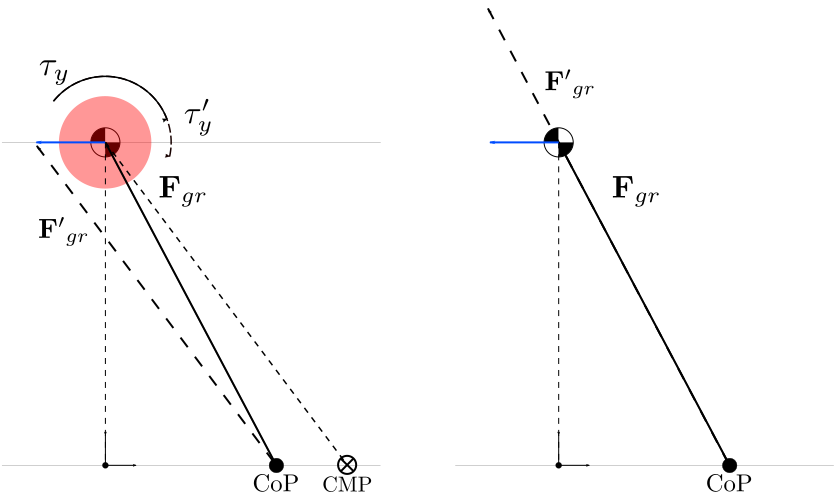
\includegraphics[width=3.2in]{modelvarzvsang2.png}
      \caption{Additional horizontal force on the CoM compared to the LIP model can be generated using angular momentum (left) and vertical motion (right). }
      \label{fig:angvsvarz}
\end{figure}

Although the use of a predefined height trajectory has many advantages, it is overly constraining. In cases where traditional balancing strategies are challenged and the robot is in risk of falling, it is interesting to explore additional capabilities of the robot to recover. Vertical CoM motion can generate additional horizontal force on the CoM, which can improve balance.

Recently, efforts have been made to use vertical motions for balance control. In \cite{koolen2016balance}, an analytic model predictive controller is derived in 2D from the \textit{orbital energy} proposed in \cite{pratt2007derivation}. Regions of attractions for this controller are studied, as well as limitations on the region in which recovery is possible under the constraint of unilateral contact only. In \cite{caron2018capturability}, a model predictive control law is proposed in 3D using sequential quadratic programming. The authors manage to solve the highly nonlinear re-planning problem online, but still make use of a relatively simple model and do not show applied results.

In this paper, we walk through the process of analyzing simple two-dimensional models from a fundamental stand point to the analyzes of the effects of those simple models in an applied setting. We propose capture regions by adding constraints to a base model. We add a contact unilaterality constraint, followed by height constraints, from which we derive analytic capture regions. We add a vertical force constraint and formulate a bang-bang control law on vertical motion, after which the solution to a capture region needs to be computed numerically. We analyze the differences of the found regions with the capture point and make a high-level comparison with angular momentum strategies. Finally, we implement the bang-bang control law in our momentum-based control framework \cite{koolen2016design}. We test push-recovery on NASA's Valkyrie \cite{radford2015valkyrie} and compare with a traditional control setup and discuss the extras that appear when going from a simple model to the robot.

The remainder of the paper is structured as follows. In Section \ref{sec:models}, we give a short overview of balancing strategies  and \textit{capture}. In Section \ref{sec:regions}, we derive capture regions for a pendulum with variable height, which are analyzed and compared with other balancing strategies in Section \ref{sec:comparison}. We test balancing on NASA's Valkyrie by applying pushes in Section \ref{sec:valkyrie}. In Section \ref{sec:discussion}, we discuss our findings and give our view on the future of balance control. Finally, in Section \ref{sec:conclusion}, we conclude.

%% MODELS
\section{BALANCE STRATEGIES \& CAPTURE}\label{sec:models}
Throughout the paper, we disregard stepping and we assume that balance strategies are dividable in:
\begin{itemize}
	\item \textit{Center of pressure strategies}: motion of the pendulum-base.
	\item \textit{Angular momentum strategies}: change of body angular momentum.
	\item \textit{Vertical motion strategies}: change of CoM height.
\end{itemize}
Furthermore, we consider cases where the use of CoP is saturated and at a constant location. Considering the a saturated CoP, additional horizontal force can be generated using \textit{angular momentum strategies} (see Fig. \ref{fig:angvsvarz}). The model to generate horizontal force, considered in this paper, is:
\begin{equation}
	\ddot{x} =\frac{x}{z}g + \frac{1}{m}\frac{\tau_y}{z},
\end{equation}
where $[x,z]$ is the CoM position in cartesian coordinates, $m$ is the body mass and $t_y$ is the torque about the CoM.

Another way to generate additional horizontal force after saturation of the CoP is the use of vertical motion. To consider vertical motions, we use the variable height pendulum model and the following dynamics are considered:
\begin{equation}
	\ddot{x} = \frac{x}{z}u,
	\label{eq:height}
\end{equation}
where $u=g+\ddot{z}$.

The goal of those strategies is to ensure \textit{balance} of the pendulum-based model: the convergence to the unstable node of the pendulum in finite time. In this paper, we use the term capture region \cite{pratt2006capture} to describe the set of footholds, where balance can be achieved. Also, the capture point as introduced by Pratt et al is considered, only this is denoted as
\begin{equation}
	x_{cp,lip} = \sqrt{\frac{z_0}{g}}\dot{x}_0
\end{equation}
for comparison. To avoid confusion, we use the term \textit{capture position} to describe a point where current state and the resulting trajectory will lead to stability of the pendulum-based model. We denote a capture position as a positive value:
\begin{equation}
	x_{cp}= |x_0|,\quad \text{if} \quad x_f=0 \wedge \dot{x}_f=0,
	\label{eq:xcp}
\end{equation}
where $x_{cp}$ is the capture position and $[x_f, \dot{x}_f]$ is the final horizontal position and velocity.

%% THEORETIC REGIONS
\section{THEORETIC CAPTURE REGIONS}\label{sec:regions}
This section proposes bounds on the capture position (\ref{eq:xcp}). The dynamics of (\ref{eq:height}) are considered. For simplicity and comparison with the LIP capture point, we take the initial vertical velocity $\dot{z}_0=0$.
\subsection{Unilateral Contact Constrained}
 Considering the constraint of unilaterality only, the capture region is bounded by the current position and the ballistic touch down point:
\begin{equation}
	x_{cp,unilateral} \in (0, x_{bal}], \quad \forall u \geq 0, 
	\label{eq:xcpuni}
\end{equation}
where $x_{bal}$ is the ballistic touchdown point and $x_{cp,unilateral}$ is the capture position under unilateral contact constraint only. The proof for this region is given in \cite{koolen2016balance}. For the zero initial height velocity, the ballistic touchdown point reads as:
\begin{equation}
 x_{bal}=t \dot{x}_0=\sqrt{\frac{2z_0}{g}}\dot{x}_0=\sqrt{2}x_{cp,lip}.
 	\label{eq:xbal}
\end{equation}

\subsection{Addition of Height Constraints}
If to the unilateral constraint CoM height constraints are added, but limitations on forces are neglected, analytic capture regions can be derived. 

Preliminary, we temporally set $\dot{z}_0 \neq 0$ to calculate the influence of an impact on $x_{cp,lip}$. Considering an initial negative vertical velocity $\dot{z}_0<0$ that is driven to zero by a vertical impact, the influence on the LIP capture point is:
\begin{align}
	x_{cp,impact} &= \sqrt{\frac{z_0}{g}}(\dot{x}_0 + \frac{x_{cp,impact}}{z_0}\dot{z}_0)\\
	&=\frac{z_0}{\sqrt{gz_0}-\dot{z}_0}\dot{x}_0, \label{eq:xcpimpact}
\end{align}
where $x_{cp,impact}$ is the impact influenced capture position from an initial impact that results in $\dot{z}=0$.

Under a minimum height constraint, we can find a capture position from which the trajectory `just' touches the constraint. We first let the mass follow the ballistic trajectory, after which it is vertically stopped by the impact influenced capture point:
\begin{equation}
	x_{cp,\zmin} = x_{bal}(\delta \zmin) + x_{cp,impact}(\zmin, \dot{z}_{\zmin}),
	\label{eq:xcpzmincomp}
\end{equation}
where $x_{cp,\zmin}$ is the capture point over the minimum height constraint, $x_{bal}(\delta \zmin)$ the horizontal position after the ballistic fall $\delta \zmin = z0-\zmin$ and $x_{cp,impact}(\zmin,\dot{z}_{\zmin}$) is $x_{cp,impact}$ after the ballistic fall. The velocity at the moment the ballistic trajectory hits the constraint is:
\begin{equation}
	\dot{z}_{\zmin} = -\sqrt{2g\delta \zmin},
\end{equation}
where $\dot{z}_{\zmin}$ is the vertical velocity at $z_{min}$. Using (\ref{eq:xcpzmincomp}), (\ref{eq:xbal}) and (\ref{eq:xcpimpact}), the capture position over the minimum height constraint reads as:
\begin{equation}
	x_{cp,\zmin} = (\sqrt{\frac{2\delta_{z_{min}}}{g}} + \frac{\zmin}{\sqrt{g \zmin}+\sqrt{2g\delta_{\zmin}}})\dot{x}_0.
\end{equation}

Also under a maximum height constraint, an analytic capture position can be found. We consider a vertical impact by the leg at $x=x_0$, which is of such magnitude that the mass is exactly at maximum height if it is slowed down by gravity. After it is slowed down, we apply $x_{cp,lip}$. This point reads as:
\begin{equation}
	x_{cp,\zmax} =(t_{\dot{z}>0} + \sqrt{\frac{\zmax}{g}})\dot{x}_{0,I}
	\label{eq:xcpzmaxcomp}
\end{equation} 
where $x_{cp,\zmax}$ is the capture position following the maximum height constraint, $t_{\dot{z}>0}$ is the time $\dot{z}>0$ and $\dot{x}_{0,I}$ is the initial velocity influenced by the impact. Note that the vertical impact that lets the mass just touch $\zmax$ is:
\begin{equation}
	\dot{z}_{I} = \sqrt{2g\delta_{\zmax}},
	\label{eq:dzi}
\end{equation}
where $\delta_{\zmax}=\zmax-z_0$. Filling in (\ref{eq:xcpzmaxcomp}) and (\ref{eq:dzi}) gives:
\begin{align}
	x_{cp,\zmax} &= (\frac{\dot{z}_I}{g}+\sqrt{\frac{\zmax}{g}})(\dot{x}_0-\frac{x_{cp,\zmax}}{z_0}\dot{z}_I)\\
	&=\frac{z_0(\sqrt{2\delta_{\zmax}}+\sqrt{\zmax})}{\sqrt{g}(z_0 + 2\delta_{\zmax} + \sqrt{2\zmax \delta_{\zmax}})}\dot{x}_0.
\end{align}

We will show that the capture positions $x_{cp,\zmin}$ and $x_{cp,\zmax}$ are also the outer bounds on the capture region.

%lem
\begin{lem}\label{lem:regionz}
Considering the dynamics of (\ref{eq:height}), $\dot{z}_0=0$, minimum height constraint $\zmin$ and maximum height constraint $\zmax$, $x_{cp,\zmin}$ and $x_{cp,\zmax}$ are the outer bounds on the capture region.
\end{lem}
%proof
\begin{proof}
For any capture position $x_{cp}$, $x\dot{x}<0$ \cite{koolen2016balance} and $0>x_0\geq-x_{bal}$ (\ref{eq:xcpuni}). 
We use that $x \leq 0, \forall t$ and $x\rightarrow 0$ along any trajectory. From (\ref{eq:height}), and $z>0$ follows that any input $u$ will slow $\dot{x}$ down. Showing that $\frac{x}{z}\rightarrow 0, \forall t$ will proof that $u=0$ for the longest possible time $t$ will lead to the farthest $x_{cp}$, and a maximum $u$ on the earliest possible $t$ will lead to the closest $x_{cp}$. 

For $u=g$, $z$ remains constant and $\frac{x}{z}\rightarrow 0$. For $u>g$, $z$ will grow and $\frac{x}{z}\rightarrow 0$. If $u<g$, we can show with the derivative of $\frac{x}{z}$ that this is always increasing:
\begin{equation}
\frac{d\frac{x}{z}}{dt}= \frac{z\dot{x}-x\dot{z}}{z^2},
\end{equation}
where $x \leq 0$ and $z \dot{x} \geq 0$. Taking the extreme case $u=0$ leads to:
\begin{align}
	z\dot{x}-x\dot{z} &= (z_0 - \frac{1}{2}gt^2)\dot{x}_0 + (x_0 + \dot{x}_0 t)gt\\
	&= (z_0 +\frac{1}{2}gt^2)\dot{x_0} + x_0gt.
\end{align}
Noting that all terms are positive except for $x_0$, which has the largest negative value for $x_0=-x_{bal}$:
\begin{align}
	(z_0 +\frac{1}{2}gt^2)\dot{x_0} - \sqrt{\frac{2z_0}{g}}\dot{x}_0gt = \dot{x}_0(\sqrt{\frac{1}{2}g}t - \sqrt{z_0})^2,
\end{align}
which is always greater than zero for all $t$.
\end{proof}

In Fig. \ref{fig:capregion}, the discussed capture regions are visualized.
\begin{figure}[h]
      \centering
      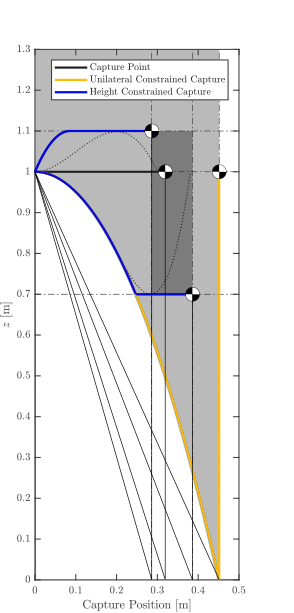
\includegraphics[width=2in]{CPLimitsDark.png}
      \caption{Visualization of the capture regions for $\dot{x}_0=1$ and $\dot{z}_0=0$. The light gray area shows the unilateral contact constrained region (\ref{eq:xcpuni}). The dark gray area shows the height constrained capture region (Lemma \ref{lem:regionz})  for $0.7<z<1.1$. The dotted plots are made with the \textit{orbital energy controller} of \cite{koolen2016balance} and show that the final points are inside the height constrained region.}
      \label{fig:capregion}
\end{figure}

\subsection{Addition of Vertical Force Constraints}\label{forcecapture}
We can also add vertical force constraints to the dynamics (\ref{eq:height}). Doing so, we assume that the robot specific limitations on joint-torque can be approximated with a minimum and maximum vertical acceleration of the CoM. Note that given Lemma 1, any extreme force at earliest convenience will lead to come closer to the height constrained limit. By inserting a constraint on vertical acceleration, an analytic solution for a capture point is not available anymore and needs to be solved numerically. 

In \cite{pratt2006capture,stephens2007humanoid,koolen2012capturability}, a bang-bang control law is used to regulate the angular momentum in the body of the model. Instead, we use a bang-bang control law for the input $u$:
\begin{multline}
	u = g + \ddot{z}_{c,1}H(t) - (\ddot{z}_{c,1} - \ddot{z}_{c,2})H(t-t_1) \\ - \ddot{z}_{c,2}H(t-t_2)),
\end{multline}
where $[\ddzcf,\ddzcs]$ are the first and second constant control inputs and have opposite signs. $H(\cdot)$ is the Heaviside function and 
\begin{equation}
t_1=\sqrt{\frac{2(z_{const}-z_0)}{\ddzcf + \frac{\ddzcf^2}{\ddzcs}}},
\end{equation}
which is the solution of:
\begin{equation}
	z_0+\frac{1}{2}\ddzcf t_1^2 + \frac{1}{2}\frac{(\ddzcf t_1)^2}{\ddzcs}= z_{const},
\end{equation}
where $z_{const}=\zmin$ if $\ddzcf <0$ and $z_{const}=\zmax$ otherwise. The time $t_2=(1-\frac{\ddzcf}{\ddzcs})t_1$, as the second `bang` needs to drive the vertical velocity of the first bang to zero. We use a binary search to find the capture positions with this control law. The cost function for this search is $|x|$ at $\dot{x}=0$. In Fig. \ref{fig:zvsf}, simulation results are shown and compared with the height constrained limits.
\begin{figure}[h]
      \centering
      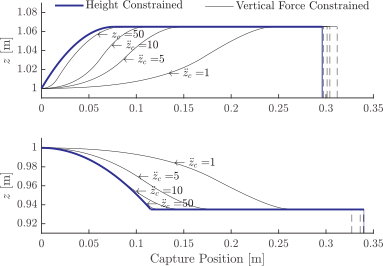
\includegraphics[width=3.3in]{heightvsforcelim2.png}
      \caption{Simulation results for the vertical force constrained capture positions for $\dot{x}_0=1$, $\dot{z}_0=0$ and $\delta \zmax=\delta \zmin=0.065$. The constant acceleration $\ddot{z}_c=\ddzcf=\ddzcs$ if $\ddot{z}_c \leq g$ and otherwise the constant with negative sign is set to $-g$. The dashed vertical lines mark the capture position. Closer to the height constrained limit means a higher value of $\ddot{z}_c$.}
      \label{fig:zvsf}
\end{figure}
%% COMPARISON
\section{Dimensional Analysis}\label{sec:comparison}
In this section we make a high-level comparison with LIP and LIP with angular momentum strategies (see Fig. \ref{fig:angvsvarz}). We use a dimensional analysis as in \cite{pratt2006capture,stephens2007humanoid,koolen2012capturability}. The following parameters are used for dimensionless position, velocity, time, inertia and hip torque:
\begin{align}
	x' &= \frac{x}{z_0}, \\
	\dot{x}' &= \frac{1}{\sqrt{gz_0}}\dot{x},\\
	t' &= t\sqrt{\frac{g}{z_0}},\\
	J' &= \frac{J}{mz_0^2},\\
	\delta x'_{cmp} &= \tau_y' = \frac{\tau_y}{mgz_0}.
\end{align}
\subsection{Limit Analysis}

\subsection{Comparison with Angular Momentum Strategy}
Also, we use an angular momentum momentum control as in \cite{pratt2006capture,stephens2007humanoid,koolen2012capturability}. The duration of each `bang` is determined using:
\begin{equation}	
	t_{1} = \sqrt{\frac{J'\theta_{max}}{\delta x'_{cmp,max}}},
\end{equation}
where $J'$ is the dimensionless inertia used in recovery, $\theta_{max}$ the maximum lunge angle of the body and $\delta x'_{cmp,max}$ the dimensionless maximum CMP offset from the CoP. Note this offset accounts for the hip torque. The average CMP offset affecting the capture position is calculated by:
\begin{equation}
 \delta x'_{cmp} = (1 -2e^{-t_1}+e^{-t_2})\delta x'_{cmp,max},
\end{equation}
where $\delta x'_{cmp}$ is the average CMP offset and $t_2=2t_1$.

We make a rough estimate of the dimensionless inertia used in recovery. We assume the CoM is located at the hip, which is also the point of rotation, and that only the body above the hip plays a role in generation of angular momentum. We model the body above the hip as a beam with mass $\frac{1}{2}m$. The length of this beam is considered equal to the CoM height. The dimensionless inertia of this beam reads as:
\begin{equation}
	J' = \frac{\frac{1}{3}(\frac{1}{2}m)z^2}{mz^2} = \frac{1}{6}.
\end{equation}
Although we make this estimate of the body inertia, we still model the body as a flywheel. Rotation of the real upper body around the hip would change the CoM height. Instead, we use a flywheel, so that the CoM is not affected by upper body `lunge'.

In Fig. \ref{fig:compare} the vertical force constrained bang-bang controller is compared with the bang-bang controller with angular momentum.

\begin{figure}[h]
      \centering
      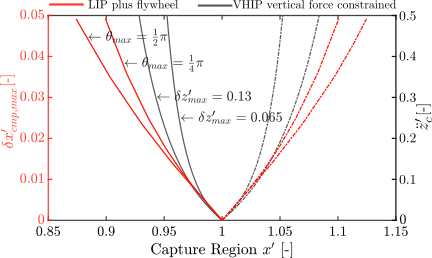
\includegraphics[width=3.3in]{capcompare.png}
      \caption{LIP model with inertia $J'=\frac{1}{6}$ versus height force constrained capture for $\dot{x}'_0=1$. For the right side of the region $\ddot{z}_c$ is initially negative for the bang bang control law.}
      \label{fig:compare}
\end{figure}
%% VALKYRIE
\section{PUSH RECOVERY ON NASA'S VALKYRIE}\label{sec:valkyrie}
In this section we apply a simple controller that uses vertical motion for balance on Valkyrie. 
\subsection{Control Law}
Our default control law is based on instantaneous capture point (ICP) \cite{koolen2012capturability} control:
\begin{equation}
	\rcmpd = \rcmpr + \mathbf{k}_{\xi}\icpe,
\end{equation}
where $\rcmpd$ is the desired CoP, $\rcmpr$ the reference CoP, $\mathbf{k}_{\xi}$ the ICP control gain and $\icpe$ is the ICP error between the reference ICP and the current ICP. For this particular test case we assume a constant $\rcmpr$, in the center of the support polygon.

The robot is controlled with a momentum-based control framework \cite{koolen2016design}, a common use in humanoid robotics \cite{kajita2003resolved, lee2012momentum}. Our framework makes use of \textit{centroidal momentum} \cite{orin2013centroidal}, the angular and linear momentum about the CoM of the robot. Desired centroidal momentum, along with motion objectives, is sent to a quadratic program, which optimizes over desired joint accelerations and desired ground reaction forces. Desired joint torques are finally computed using an inverse-dynamics algorithm. We typically only select the linear part of the desired momentum rate for control. The desired horizontal linear momentum rate is computed as:
\begin{equation}
	\dot{\mathbf{l}}_{d,xy} = \frac{\mathbf{c}_{xy}-\rcmpd}{z}(mg + \dot{\mathbf{l}}_{d,z}),
\end{equation}
where $\mathbf{c}_{xy}=[x,y]$ and $\dot{\mathbf{l}}_{d} \in \mathbb{R}^3$ is the desired linear momentum rate of change. Note that with little vertical motion, $ \dot{\mathbf{l}}_{d,z}$ is small.

Normally during the stance phase, like we consider, the height is controlled to a default constant reference height. In this experiment, we use a similar control law for vertical acceleration as the bang-bang controller in Section \ref{forcecapture}. The following parameters are used for the controller in addition to the already discussed constraints:
\begin{itemize}
	%\item $\alpha_{\icpe}^+$: Threshold to turn the controller on $|\icpe|>\alpha_{\icpe}^+$, which for example can be tuned to activate the controller when $\rcmpd$ is near the edge of the polygon. 
	%\item $\alpha_{\icpe}^-$: Threshold to turn the controller off $|\icpe|<\alpha_{\icpe}^-$, when the robot is back to stability.
	\item $\dddot{z}_{max}$: Maximum allowed vertical CoM jerk.
	\item $\alpha_{\hat{\ddot{z}}_{c}}$: Parameter to scale down expected $\ddot{z}_c$ for the second `bang', due to jerk limits.
\end{itemize}

The control sequence we use for the bang-bang controller reads as follows. For the first `bang': $\ddot{z}_d=\ddot{z}_c$. The transition from the first `bang` to the second is if:
\begin{equation}
	z+\frac{1}{2}\frac{\dot{z}^2}{\alpha_{\hat{\ddot{z}}_{c}}\ddot{z}_{c}} >\zmax,
\end{equation}
in the case of approaching a maximum height. This results in $\ddot{z}_d=-\ddot{z}_c$ until $\dot{z}<0$, after which the height is controlled to $\zmax$ until the controller turns off:
\begin{equation}
	\ddot{z}_d = k_p(z_r-z)-k_d\dot{z},
\end{equation}
where $[k_p,k_d]=[50.0,14.0]$ are the PD-control gains and reference height $z_r= \zmax$. If the controller is turned off, the height is controlled to the default height and $z_r=z_0$.
\subsection{Experimental Setup}
We test push recovery on Valkyrie during stance phase, by applying a push from the back at chest height. The following parameter values are chosen to work with:
\begin{itemize}
\item $z_0=1.01$ [m], our default reference CoM height during stance.
\item $\zmax=1.065$ [m], the maximum CoM height during stance, such that the legs are not in singular configuration.
\item $\dddot{z}_{max} = 80.0$ [m/s3]
\item $\ddot{z}_c=2.4$ [m/s2], a value that found to work `well' on hardware. E.g., higher values would result in the robot to shake.
\end{itemize}

Additionally, whole-body controller parameters relevant to the test setup are given in Tab. \ref{tab:params}. For the angular motion objectives, the desired is generated with PD-control about a constant reference with $[k_p, k_d]=[100.0,16.0]$. The quadratic program uses an active-set solver.
\begin{table}[h]
\caption{Relevant whole-body control parameters}
\label{tab:params}
\begin{center}
\begin{tabular}{llc}
\hline~\\[-2ex]
\textbf{Task group} & \textbf{Task} & \textbf{Weight}\\
\hline ~\\[-2ex]
Momentum linear& $X$ & $5 \cdot 10^{-2}$\\
Momentum linear& $Z$ & $1 \cdot 10^{-2}$\\
Motion angular& Chest &    $1.5 \cdot 10^1$\\
Motion angular& Pelvis &  $5 \cdot 10^0$\\
Motion angular& Support foot &  $5 \cdot 10^0$\\
Regularization & Basis vector multiplier&  $1 \cdot 10^{-5}$\\
Regularization & Multiplier rate & $5 \cdot 10^{-8}$\\
Regularization & Joint acceleration & $5 \cdot 10^{-3}$\\
Regularization & Joint jerk & $1.6 \cdot 10^{-6}$\\
\hline
\end{tabular}
\end{center}
\end{table}

\subsection{Simulation Results}
For simulation tests, we used a value of $\alpha_{\hat{\ddot{z}}_{c}}=0.4$ for the influence of jerk limitations. The push duration is $0.15$ [s]. We compare the default control setup with the controller that uses vertical motion. 

\subsubsection{Analysis}
The maximum recoverable push for the default control setup is $34.5$ [Ns] for the given push duration. The vertical motion controller still recovered after a push of $37.6$ [Ns]. In Fig. \ref{fig:valcomparephase}, a phase plot is shown for the two push magnitudes for both control setups. The default setup loses stability at the larger push. With the smaller push, the vertical motion controller has a considerably smaller area than the default control setup.
\begin{figure}[h]
      \centering
      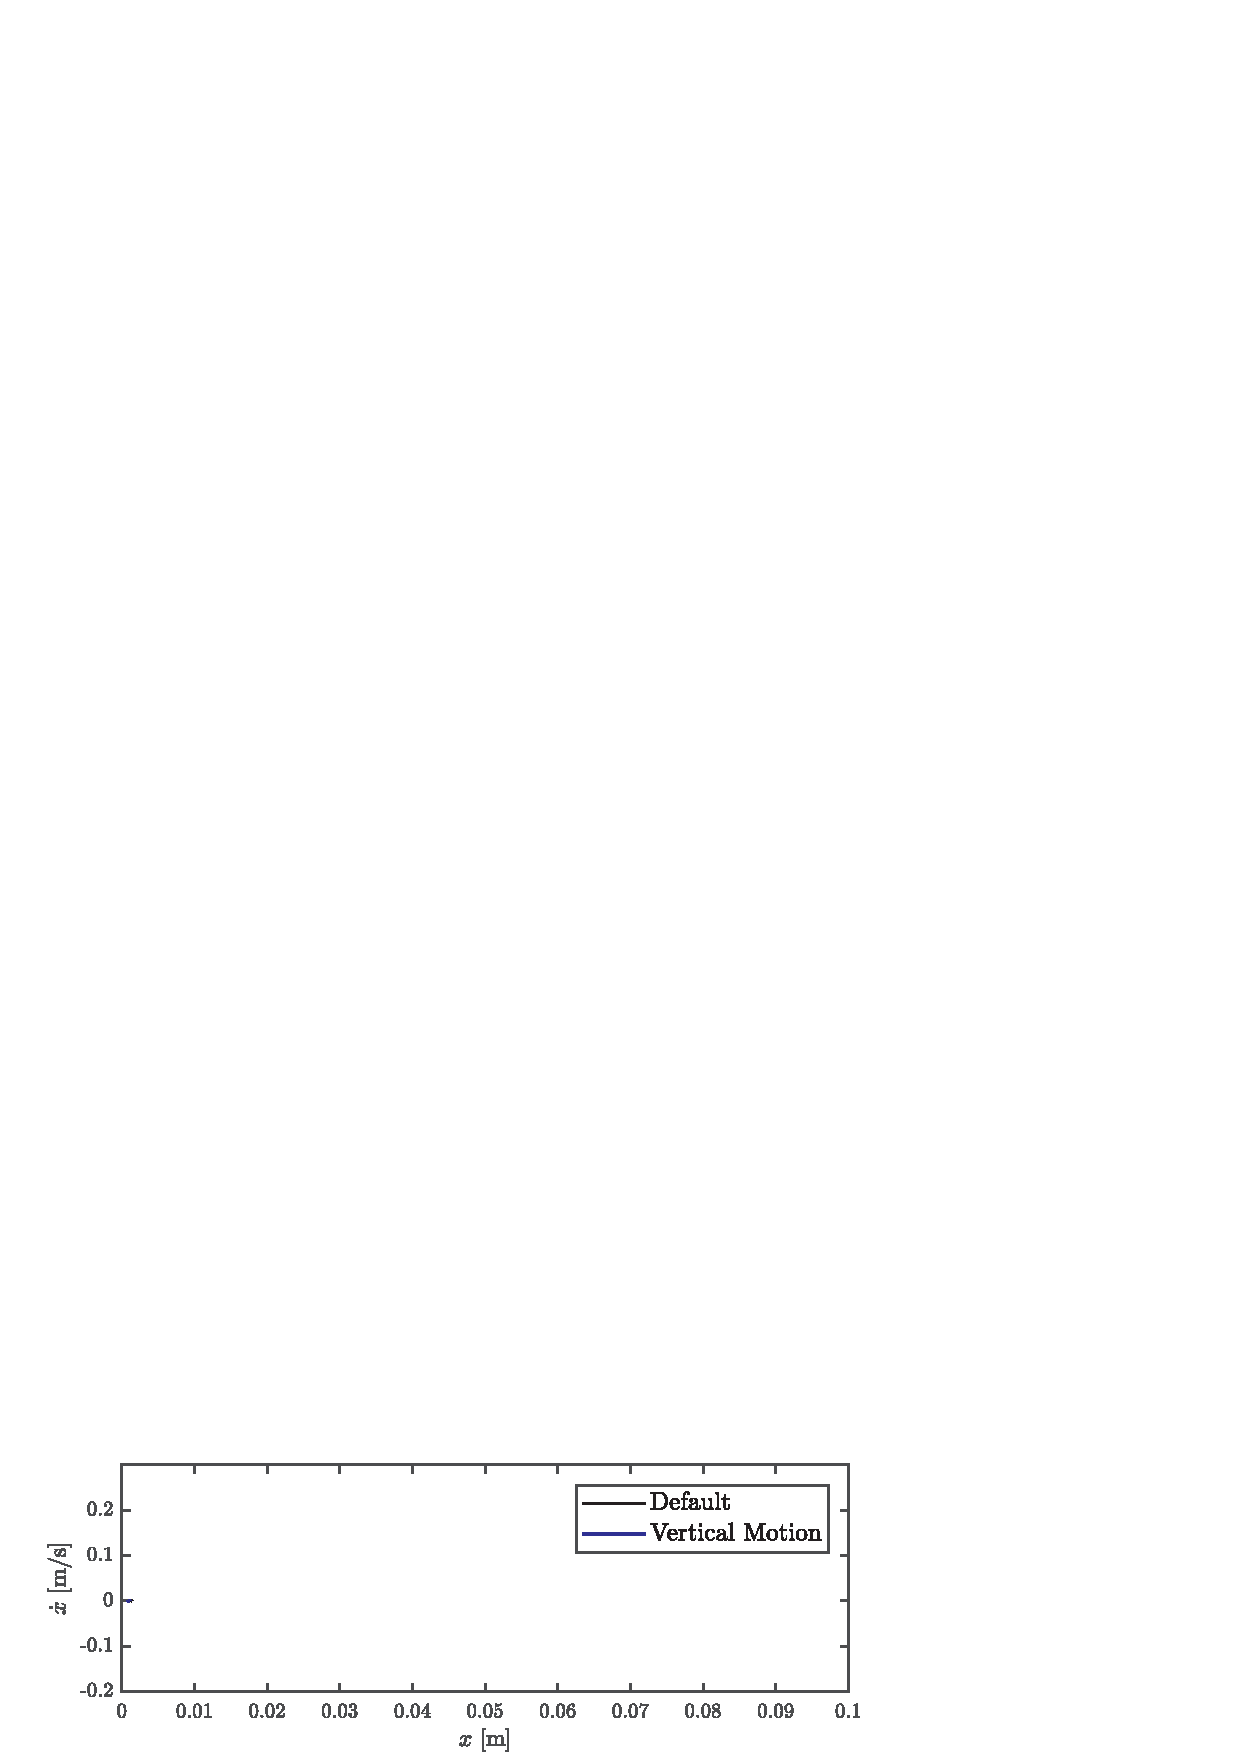
\includegraphics[width=3.3in]{valcomparephase.png}
      \caption{Phase plot of a push of $34.5$ [Ns] (solid) and a push of $37.6$ [Ns] (dotted).}
      \label{fig:valcomparephase}
\end{figure}

We analyzed the differences in resulting joint torques and noticed that the difference in ankle torque is the largest amount. Furthermore, we found it interesting to compare the rotation error of the torso. Angular momentum `strategies' commonly result in rotation of the upper body. We want to include this rotation in our analysis, as not rotating the body might be one of the advantages of vertical motion.  In Fig. \ref{fig:valcompare}, centroidal momentum rate, CoM height, torso rotation and ankle torque plots over time are shown. The achieved vertical linear momentum rates have a little overshoot for both controllers. This may also be a reason for the overshoot in height in the fourth graph in the figure. Controversially, the achieved horizontal linear momentum rate is lower than the desired for both controllers. In the first $0.25$ [s], the vertical motion controller achieves almost double the horizontal momentum rate than the default controller. The differences in achieved angular momentum rate are relatively small, as well as the differences in torso rotation. The peak ankle torque is about $25\%$ higher with the vertical motion controller.
\begin{figure}[h]
      \centering
      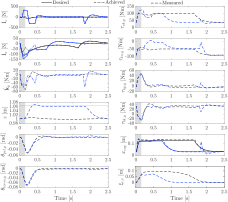
\includegraphics[width=3.3in]{valcomparetime.png}
      \caption{Comparison of push recovery between the default setup (black) versus the vertical motion controller (blue) for a push of $34.5$ [Ns]. The gray area is where the push is applied. }
      \label{fig:valcompare}
\end{figure}

\subsubsection{Comparison with Capture Regions}
The increase in recovery of the vertical motion controller is about $9\%$ compared to the default control setup. The force constrained capture point for the same $\ddot{z}_c$ and $\zmax$ is only about $4\%$ smaller than $x_{cp,lip}$, which is a remarkable difference. From the results in Fig. \ref{fig:valcompare}, we assume that a difference in angular momentum is not a reason for this. Also, we noticed that joint angle limits and joint acceleration limits where not violated during the tests.
However, the difference in the achieved horizontal momentum rate is large. Note that this is a result of the momentum-based control framework. Generation of horizontal linear momentum rate may conflict with other objectives, such as keeping the upper body straight, and maintaining a certain height.

\subsection{Hardware Results}
We tested the same two setups on hardware as in simulation. We only used a value of $\alpha_{\hat{\ddot{z}}_{c}}=0.8$, which appeared to be a better `estimate' for reaching the maximum height for the vertical motion controller.

We compared two times a dozen test samples that the robot `just' recovered from the applied push, which we define as the CoM coming closer than $5.0$ [mm] from the polygon edge. We measured the push force with an iLoad Pro Digital load sensor at its maximum record frequency of $100$ [Hz]. In Fig. \ref{fig:impulsecompare}, the average force profiles with standard deviation for both control setups are graphed. The values for the integrated push force are very similar to the simulation results. However, the measured force profile on hardware is different from the profile of the constant force applied in simulation. In Fig. \ref{fig:val}, a time-lapse image is shown from Valkyrie recovering from a push using the vertical motion controller.

\begin{figure}[h]
      \centering
      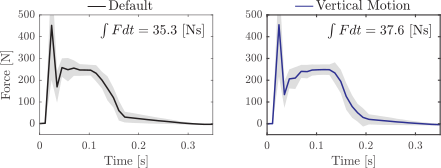
\includegraphics[width=3.3in]{impulsecompare.png}
      \caption{Average push force profiles of 12 pushes where the CoM went closer than $5.0$ [mm] from the polygon edge. The gray area is the standard deviation above and below the graph. }
      \label{fig:impulsecompare}
\end{figure}


\section{DISCUSSION AND FUTURE WORK}\label{sec:discussion}
\subsection{From Flywheel Model to Real Robot}
\subsection{3D Control}

\section{CONCLUSION}\label{sec:conclusion}
\begin{figure*}[h]
\centering
  \begin{tabular}{cccc}
    \includegraphics[width=1.6in]{val1} &
    \includegraphics[width=1.6in]{val3} &
    \includegraphics[width=1.6in]{val5} &
    \includegraphics[width=1.6in]{val8} \\
  \end{tabular}
  \caption{Time-lapse of Valkyrie recovering from a push using vertical motion.}
  \label{fig:val}
\end{figure*}

\addtolength{\textheight}{-12cm}   % This command serves to balance the column lengths
                                  % on the last page of the document manually. It shortens
                                  % the textheight of the last page by a suitable amount.
                                  % This command does not take effect until the next page
                                  % so it should come on the page before the last. Make
                                  % sure that you do not shorten the textheight too much.


\bibliographystyle{IEEEtran}
\bibliography{IEEEabrv,IEEEexample}



\end{document}
